\section*{Analiza porównacza wyjaśnień}
W tej sekcji przeprowadzimy analizę porównawcą wyjaśnień generowanych przez różne metody XAI: LIME, SHAP i GradCAM.
Oceny dokonamy na podstawie Iou oraz zmian pewności modelu.
Analiza zostaine przeprowadzona na całym zbiorze danych, a następnie z podziełem na kategorie obrazów oraz w zależności od wielkości obiektów.

\textbf{Analiza na całym zbiorze danych}.
W tej części przeprowadzimy analizę porównawczą metod XAI na całym zbiorze danych.
Skupimy się na ocenie Intersection over Union oraz zmianach w pewności modelu po zastosowaniu wyjaśnień. Celem jest zrozumienie, jak skutecznie każda metoda identyfikuje istotne cechy obrazu w kontekście całego zbioru.

\begin{figure}
	\centering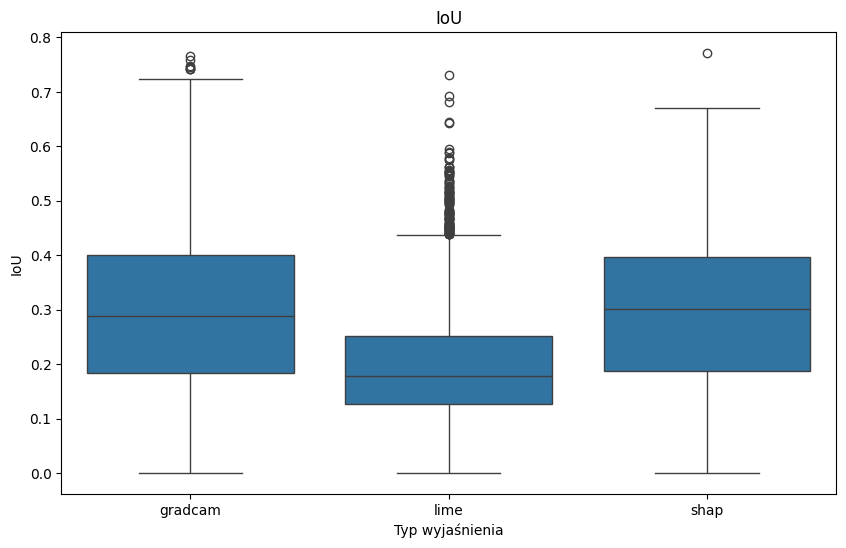
\includegraphics[width=.6\textwidth]{img/base_iou}
	\caption{Wartości IoU  dla stosowanych obrazów}  \label{rys:basiciou}
\end{figure}
Najwyższą średnią wartość IoU osiągnął GradCAM z wartością 0.298 oraz SHAP z wartością 0.292, natomiast najgorszą osiągnął LIME z wartością średnią 0.199.
Na rys \ref{rys:basiciou} widnieje wykres pudełkowy.

\begin{figure}
	\centering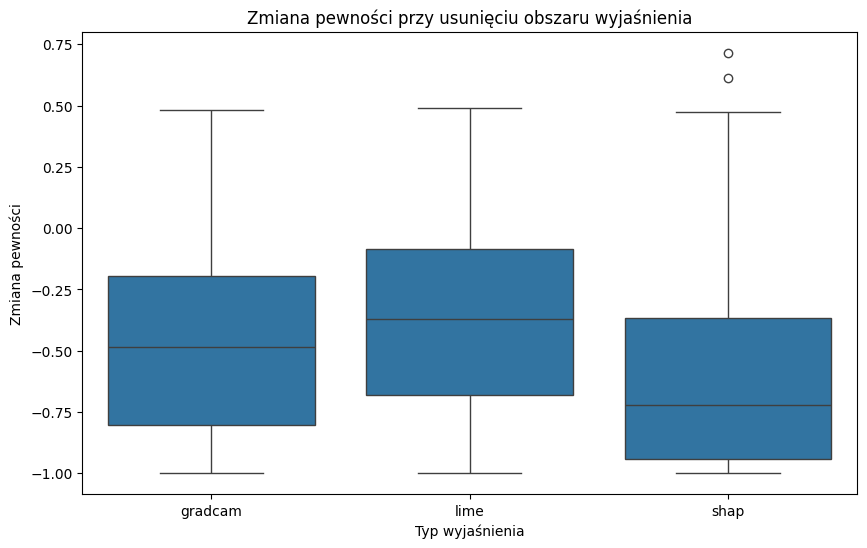
\includegraphics[width=.6\textwidth]{img/base_confidence_mask}
	\caption{Zmiana pewności przy usunięcu obszarów wyjaśnienia}  \label{rys:base_confidence_mask}
\end{figure}

Im bardziej się zmniejszyła pewność modelu tym ważniejszy był obszar wyjaśnienia.
Metodą która wpłyneła w negatywny sposób na pewność modelu jest SHAP z śrenią zmianą -0.622, następnie GradCAM ze średnim wynikiem -0.491 oraz LIME z -0.400.
Na \ref{rys:base_confidence_mask} widać wykres pudełkowy, na którym widzimy że usuniecie obszarów wyjaśnień prawie zawsze zmniejszało pewność, z pewnymi wyjątkami.

Average Percent Increase in Confidence
\begin{figure}
	\centering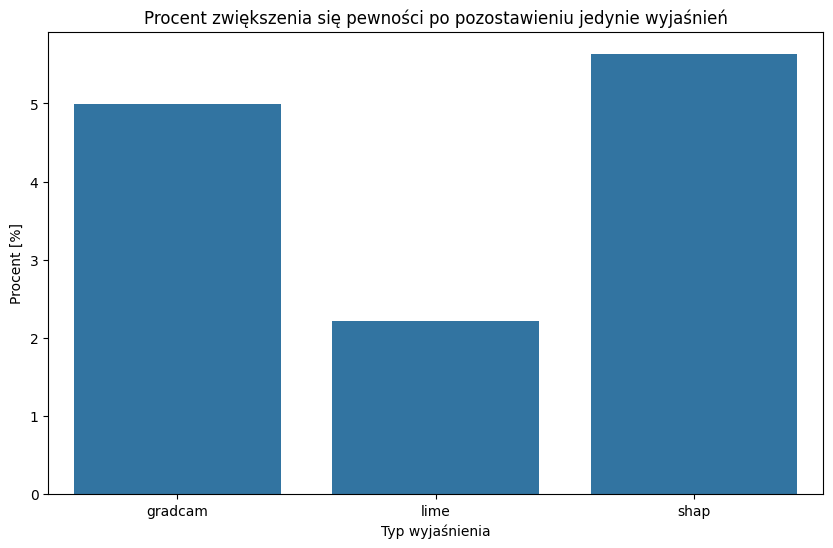
\includegraphics[width=.6\textwidth]{img/base_confidence_womask_percent}
	\caption{Procent zwiękeszenia się pewności po pozostawieniu jedynie obszarów wyjaśnień}  \label{rys:base_confidence_womask_percent}
\end{figure}

Na rys \ref{rys:base_confidence_womask_percent} widać wykres, przedstawiający jaka część predykcji zwiększyłą się po pozostawieniu jedynie obszarów wyjaśnień.
Największym procentem, co za tym idzie najlepszym wynikiem jest SHAP z 5.630\%, następnie GradCAM z 4.988\% i nagorszym wynikiem LIME 2.222\%.

\subsection*{Kategorie}

\textbf{Analiza w zależności od klasy obrazów}.
W tej części dokonamy analizy porównawczej metod XAI z uwzględnieniem różnych kategorii obrazów.
Porównamy skuteczność wyjaśnień generowanych przez LIME, SHAP i GradCAM dla różnych klas.
Celem jest ocena, jak metody radzą sobie w kontekście specyficznych rodzajów obrazów.

\begin{figure}
	\centering
	\begin{minipage}[b]{0.3\textwidth}
		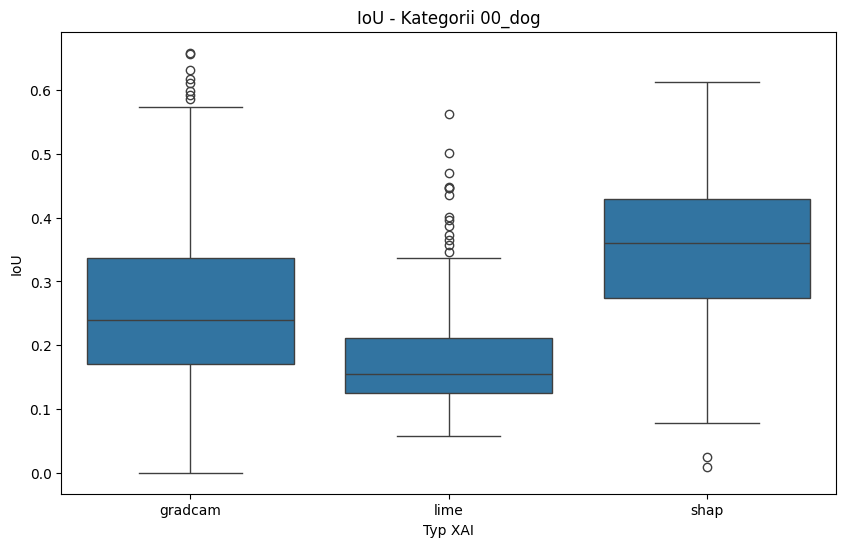
\includegraphics[width=.9\textwidth]{img/base_iou_dog}
		\caption{Wartość IoU wyjaśnień dla kategorii Dog}  \label{rys:base_iou_dog}
	\end{minipage}
	\begin{minipage}[b]{0.3\textwidth}
		\centering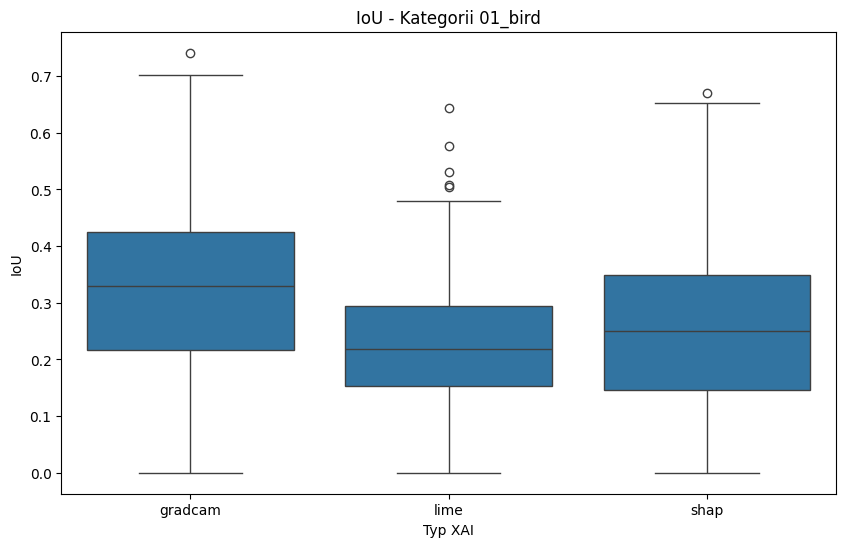
\includegraphics[width=.9\textwidth]{img/base_iou_bird}
		\caption{Wartość IoU wyjaśnień dla kategorii Bird}  \label{rys:base_iou_bird}
	\end{minipage}
	\begin{minipage}[b]{0.3\textwidth}
		\centering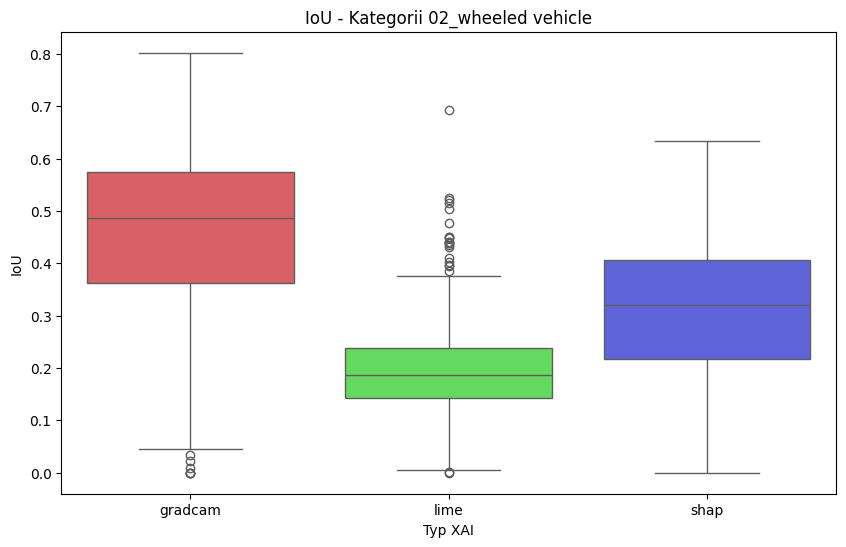
\includegraphics[width=.9\textwidth]{img/base_iou_vehicle}
		\caption{Wartość IoU wyjaśnień dla kategorii Vehicle}  \label{rys:base_iou_vehicle}
	\end{minipage}
\end{figure}
\begin{figure}
	\centering
	\begin{minipage}[b]{0.3\textwidth}
		\centering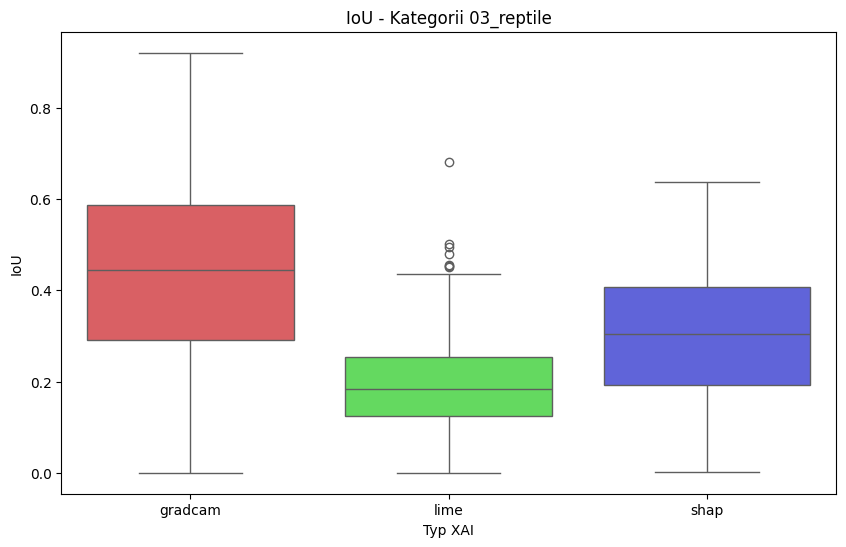
\includegraphics[width=.9\textwidth]{img/base_iou_reptile}
		\caption{Wartość IoU wyjaśnień dla kategorii Reptile}  \label{rys:base_iou_reptile}
	\end{minipage}
	\begin{minipage}[b]{0.3\textwidth}
		\centering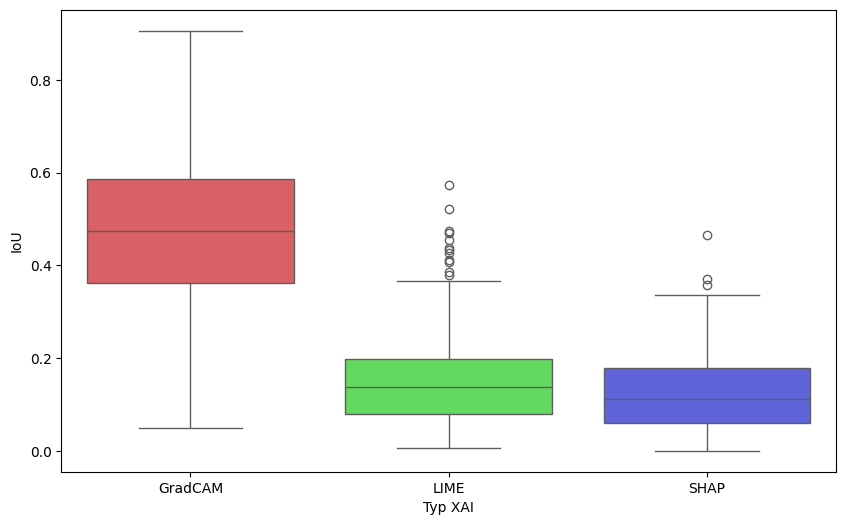
\includegraphics[width=.9\textwidth]{img/base_iou_carnivore}
		\caption{Wartość IoU wyjaśnień dla kategorii Carnivore}  \label{rys:base_iou_carnivore}
	\end{minipage}
	\begin{minipage}[b]{0.3\textwidth}
		\centering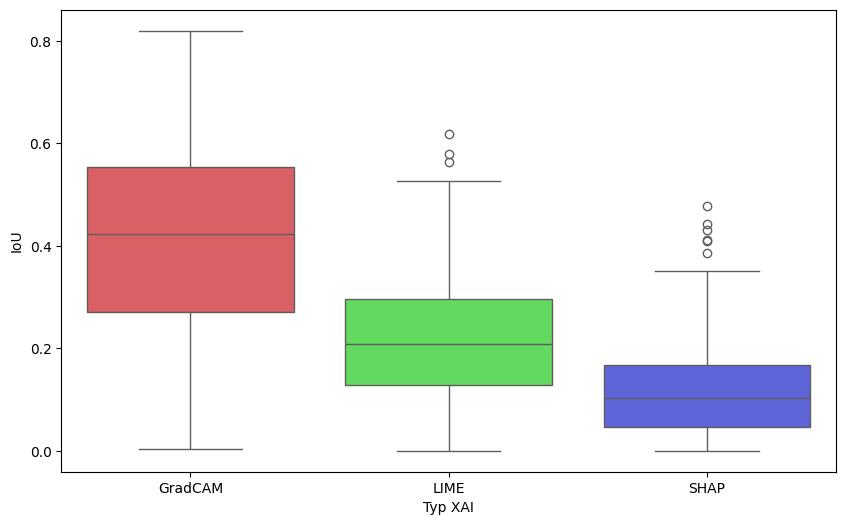
\includegraphics[width=.9\textwidth]{img/base_iou_insect}
		\caption{Wartość IoU wyjaśnień dla kategorii Insect}  \label{rys:base_iou_insect}
	\end{minipage}
\end{figure}
\begin{figure}
	\centering
	\begin{minipage}[b]{0.3\textwidth}
		\centering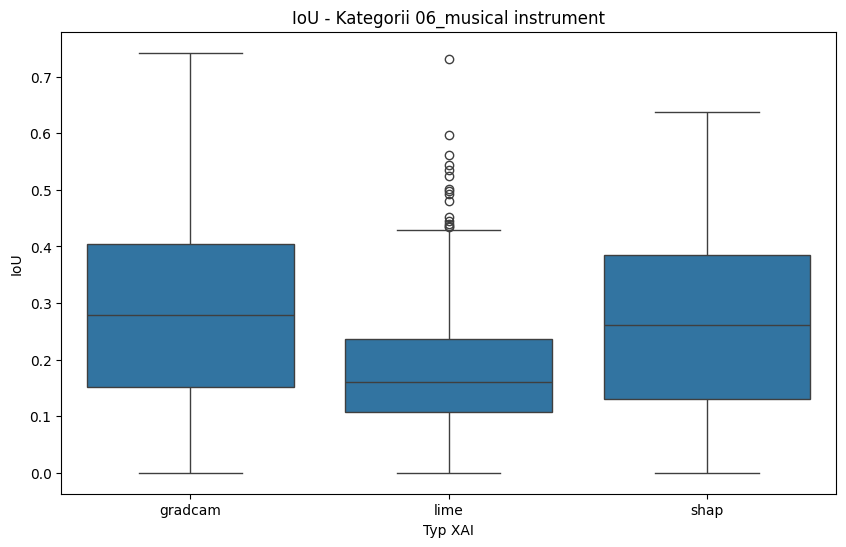
\includegraphics[width=.9\textwidth]{img/base_iou_music}
		\caption{Wartość IoU wyjaśnień dla kategorii Instrument}  \label{rys:base_iou_music}
	\end{minipage}
	\begin{minipage}[b]{0.3\textwidth}
		\centering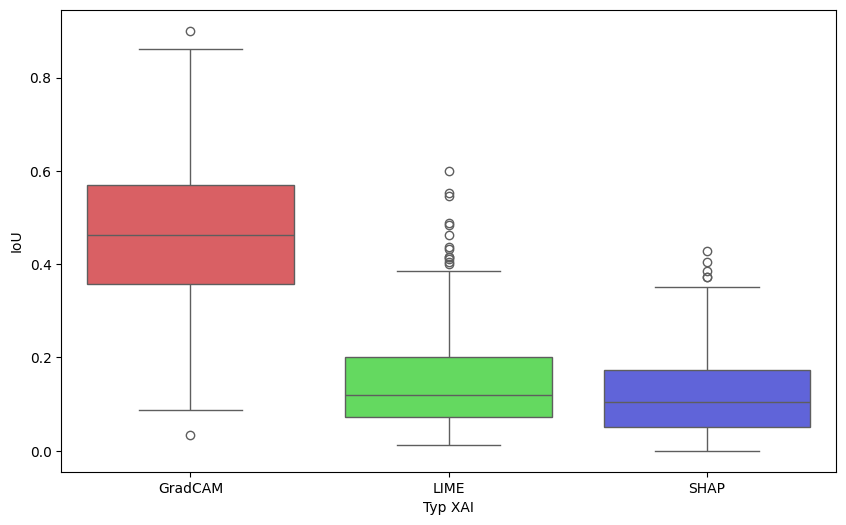
\includegraphics[width=.9\textwidth]{img/base_iou_primate}
		\caption{Wartość IoU wyjaśnień dla kategorii Primate}  \label{rys:base_iou_primate}
	\end{minipage}
	\begin{minipage}[b]{0.3\textwidth}
		\centering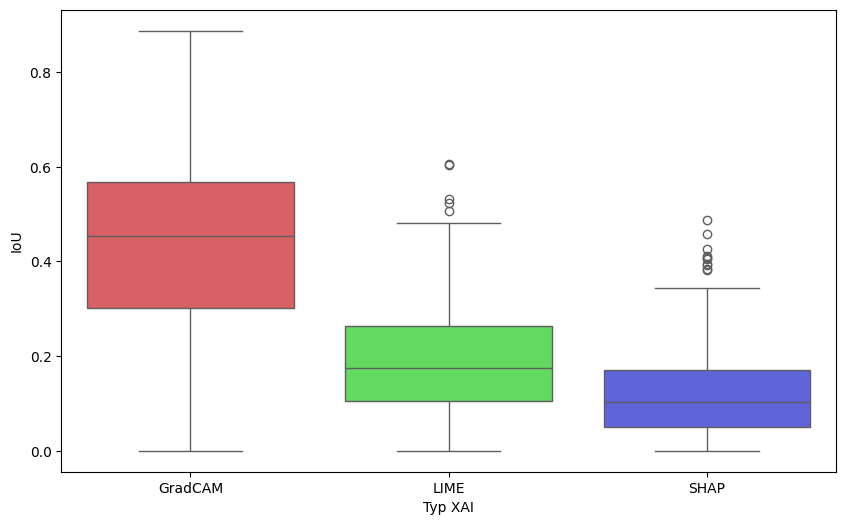
\includegraphics[width=.9\textwidth]{img/base_iou_fish}
		\caption{Wartość IoU wyjaśnień dla kategorii Fish}  \label{rys:base_iou_fish}
	\end{minipage}
\end{figure}
Porównując IoU dla różnych kategori jesteśmy w stanie zobaczyć, że LIME posiada najniższą medianę dla każdej kategorii, natomiast SHAP oraz GradCAM posiadają lepsze wyniki w zależności od dobranej kategorii.
SHAP posiada widocznie lepsze wyniki dla kategorii: Carnivore (\ref{rys:base_iou_carnivore}), Dog(\ref{rys:base_iou_dog}), Primate(\ref{rys:base_iou_primate}).
Natomiast GradCAM posiada widocznie lepsze wyniki dla kategorii: Fish(\ref{rys:base_iou_fish}), Insect(\ref{rys:base_iou_insect}), Bird(\ref{rys:base_iou_bird}).

\begin{figure}
	\centering
	\begin{minipage}[b]{0.3\textwidth}
		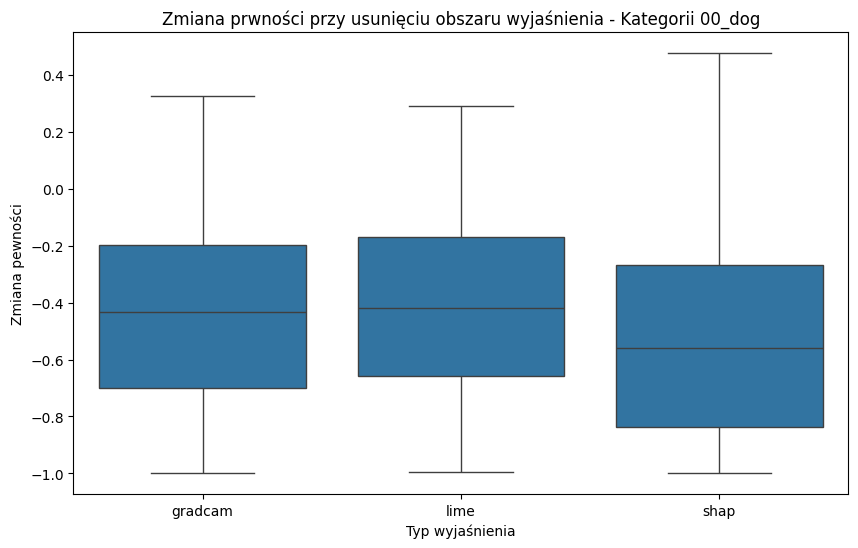
\includegraphics[width=.9\textwidth]{img/base_confidence_mask_dog}
		\caption{Wartość IoU wyjaśnień dla kategorii Dog}  \label{rys:base_confidence_mask_dog}
	\end{minipage}
	\begin{minipage}[b]{0.3\textwidth}
		\centering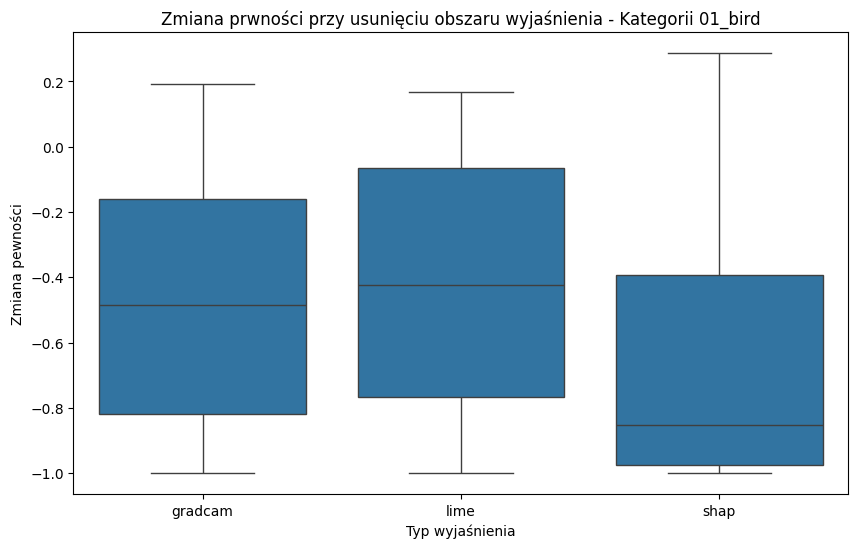
\includegraphics[width=.9\textwidth]{img/base_confidence_mask_bird}
		\caption{Wartość IoU wyjaśnień dla kategorii Bird}  \label{rys:base_confidence_mask_bird}
	\end{minipage}
	\begin{minipage}[b]{0.3\textwidth}
		\centering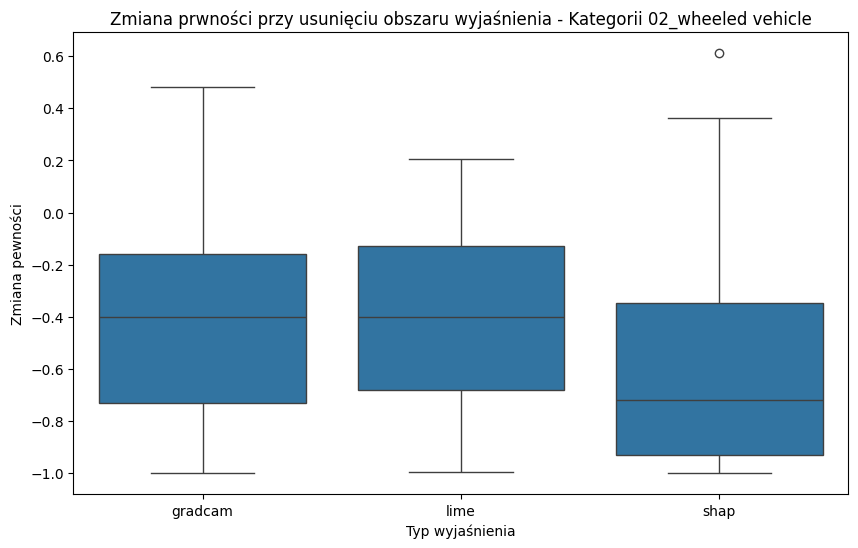
\includegraphics[width=.9\textwidth]{img/base_confidence_mask_vehicle}
		\caption{Wartość IoU wyjaśnień dla kategorii Vehicle}  \label{rys:base_confidence_mask_vehicle}
	\end{minipage}
\end{figure}
\begin{figure}
	\centering
	\begin{minipage}[b]{0.3\textwidth}
		\centering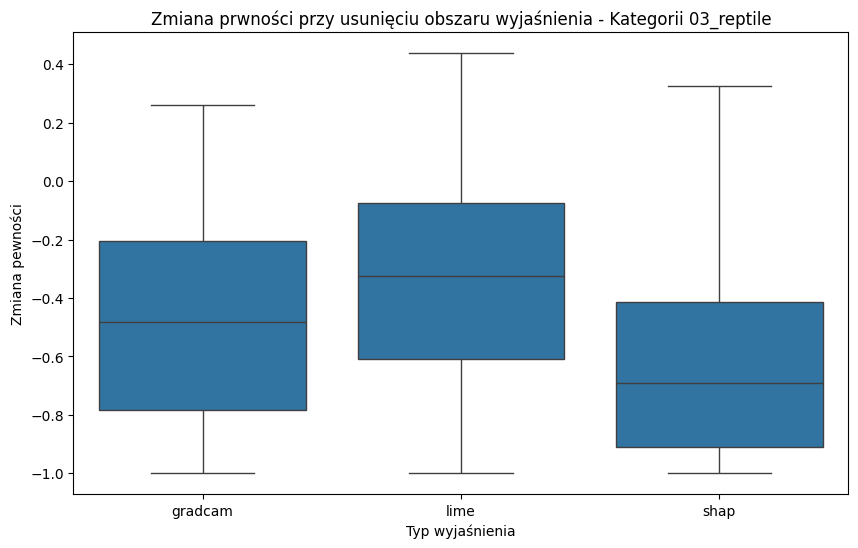
\includegraphics[width=.9\textwidth]{img/base_confidence_mask_reptile}
		\caption{Wartość IoU wyjaśnień dla kategorii Reptile}  \label{rys:base_confidence_mask_reptile}
	\end{minipage}
	\begin{minipage}[b]{0.3\textwidth}
		\centering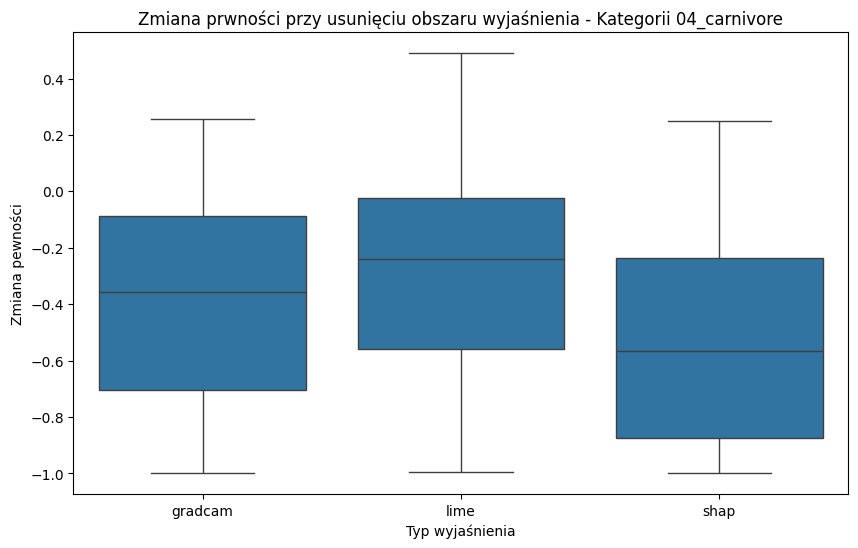
\includegraphics[width=.9\textwidth]{img/base_confidence_mask_carnivore}
		\caption{Wartość IoU wyjaśnień dla kategorii Carnivore}  \label{rys:base_confidence_mask_carnivore}
	\end{minipage}
	\begin{minipage}[b]{0.3\textwidth}
		\centering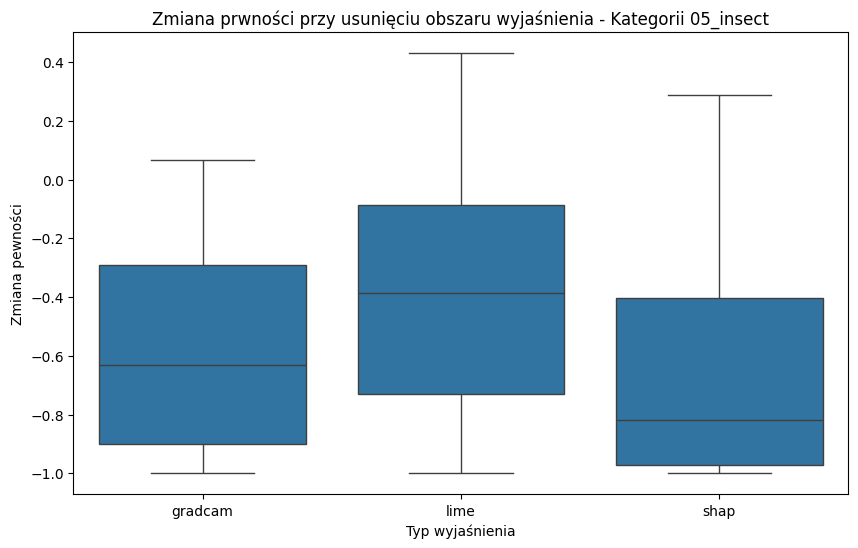
\includegraphics[width=.9\textwidth]{img/base_confidence_mask_insect}
		\caption{Wartość IoU wyjaśnień dla kategorii Insect}  \label{rys:base_confidence_mask_insect}
	\end{minipage}
\end{figure}
\begin{figure}
	\centering
	\begin{minipage}[b]{0.3\textwidth}
		\centering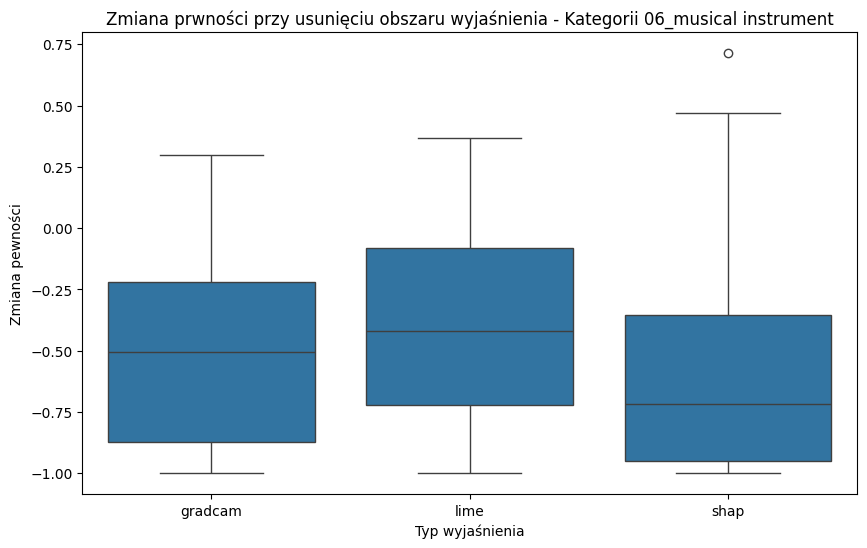
\includegraphics[width=.9\textwidth]{img/base_confidence_mask_music}
		\caption{Wartość IoU wyjaśnień dla kategorii Instrument}  \label{rys:base_confidence_mask_music}
	\end{minipage}
	\begin{minipage}[b]{0.3\textwidth}
		\centering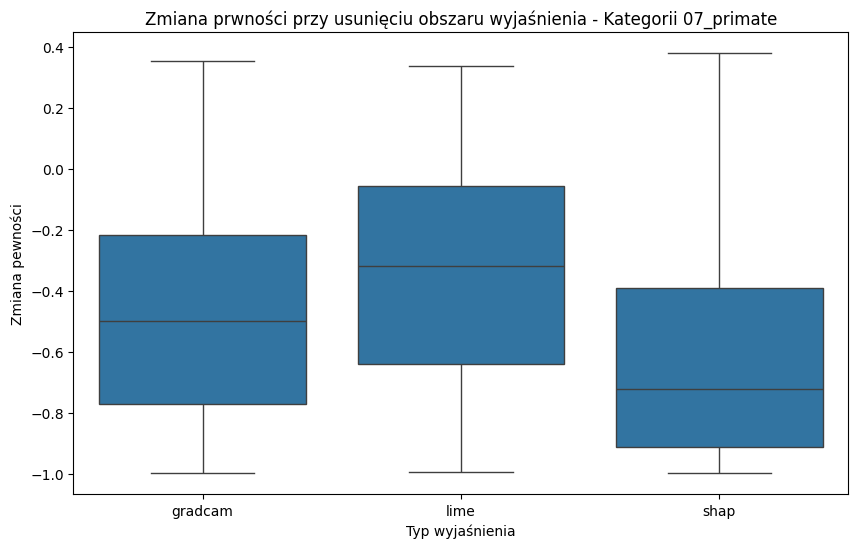
\includegraphics[width=.9\textwidth]{img/base_confidence_mask_primate}
		\caption{Wartość IoU wyjaśnień dla kategorii Primate}  \label{rys:base_confidence_mask_primate}
	\end{minipage}
	\begin{minipage}[b]{0.3\textwidth}
		\centering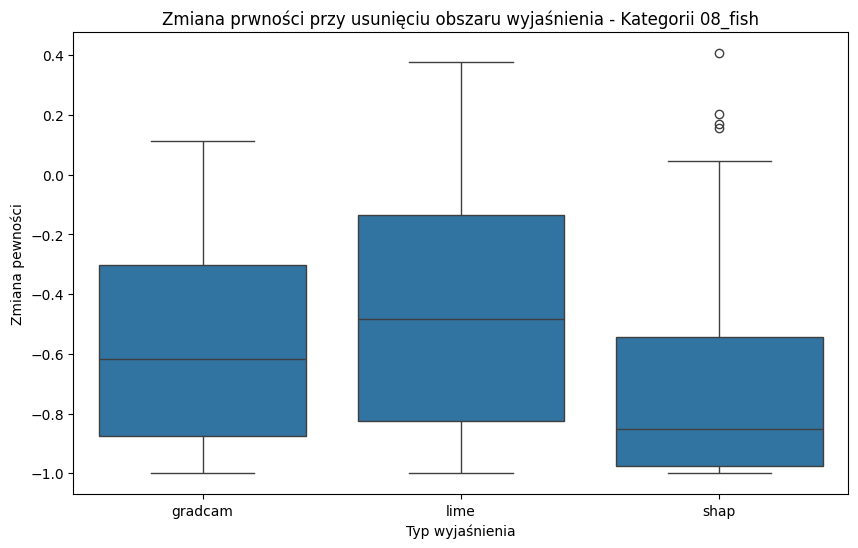
\includegraphics[width=.9\textwidth]{img/base_confidence_mask_fish}
		\caption{Wartość IoU wyjaśnień dla kategorii Fish}  \label{rys:base_confidence_mask_fish}
	\end{minipage}
\end{figure}
Największą negatywną zmianą jest zawsze dla SHAPA niezależnie od kategorii, następnie dla GradCAM a na końcu dla lime, dla wszystkich poza Vehicle(\ref{rys:base_confidence_mask_vehicle}) oraz Dog(\ref{rys:base_confidence_mask_dog}) gdzie LIME oraz GradCAM są na podobnym poziomie.

\begin{figure}
	\centering
	\begin{minipage}[b]{0.3\textwidth}
		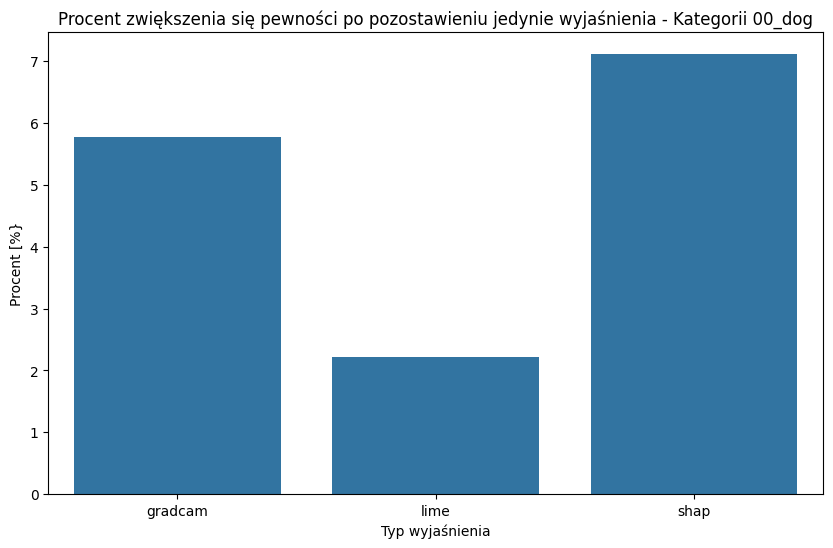
\includegraphics[width=.9\textwidth]{img/base_confidence_womask_percent_dog}
		\caption{Procent zwiększenia się pewności po pozostawieniu jedynie wyjaśnienia - Kategoria Dog}  \label{rys:base_confidence_womask_percent_dog}
	\end{minipage}
	\begin{minipage}[b]{0.3\textwidth}
		\centering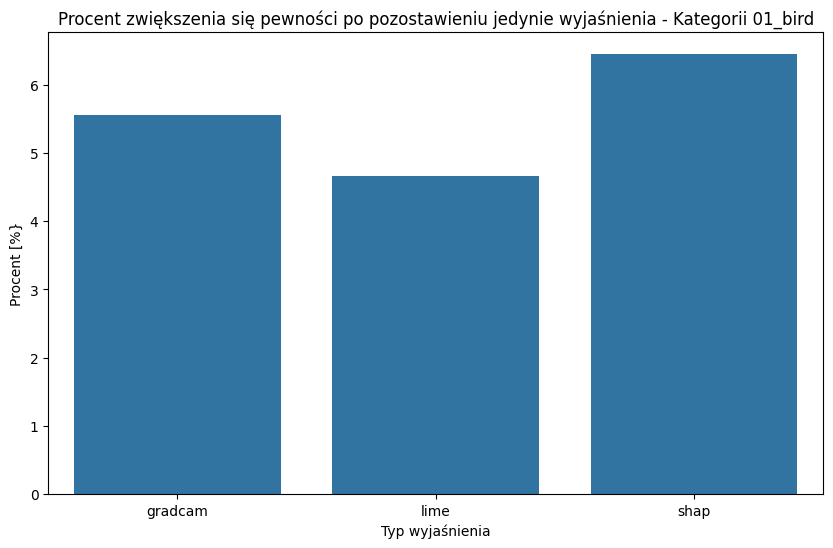
\includegraphics[width=.9\textwidth]{img/base_confidence_womask_percent_bird}
		\caption{Procent zwiększenia się pewności po pozostawieniu jedynie wyjaśnienia - Kategoria Bird}  \label{rys:base_confidence_womask_percent_bird}
	\end{minipage}
	\begin{minipage}[b]{0.3\textwidth}
		\centering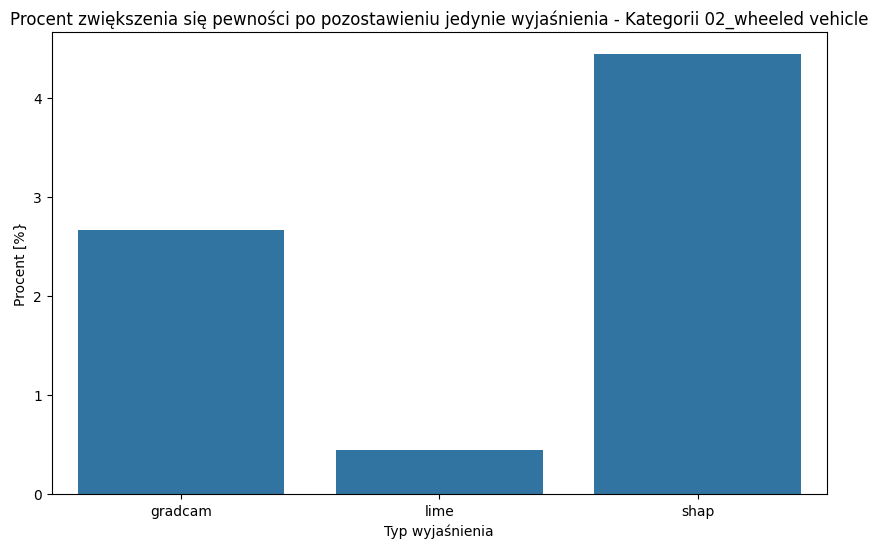
\includegraphics[width=.9\textwidth]{img/base_confidence_womask_percent_vehicle}
		\caption{Procent zwiększenia się pewności po pozostawieniu jedynie wyjaśnienia - Kategoria Vehicle}  \label{rys:base_confidence_womask_percent_vehicle}
	\end{minipage}
\end{figure}
\begin{figure}
	\centering
	\begin{minipage}[b]{0.3\textwidth}
		\centering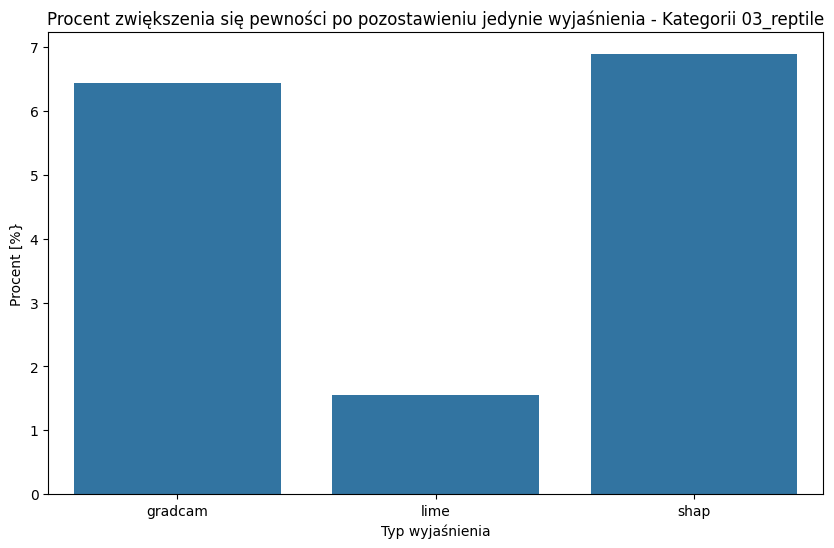
\includegraphics[width=.9\textwidth]{img/base_confidence_womask_percent_reptile}
		\caption{Procent zwiększenia się pewności po pozostawieniu jedynie wyjaśnienia - Kategoria Reptile}  \label{rys:base_confidence_womask_percent_reptile}
	\end{minipage}
	\begin{minipage}[b]{0.3\textwidth}
		\centering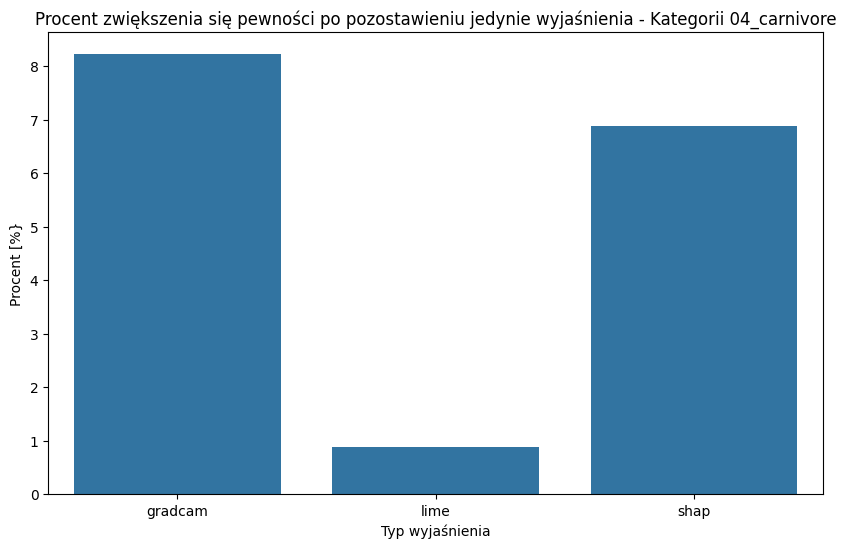
\includegraphics[width=.9\textwidth]{img/base_confidence_womask_percent_carnivore}
		\caption{Procent zwiększenia się pewności po pozostawieniu jedynie wyjaśnienia - Kategoria Carnivore}  \label{rys:base_confidence_womask_percent_carnivore}
	\end{minipage}
	\begin{minipage}[b]{0.3\textwidth}
		\centering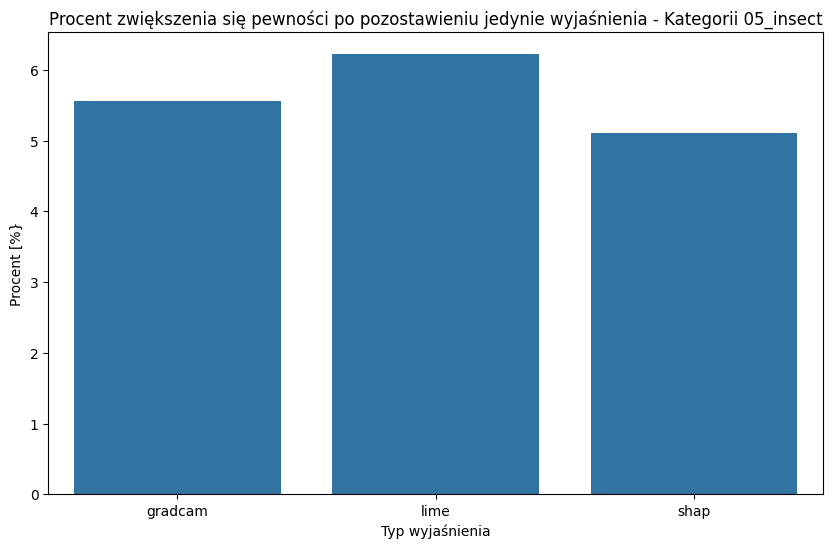
\includegraphics[width=.9\textwidth]{img/base_confidence_womask_percent_insect}
		\caption{Procent zwiększenia się pewności po pozostawieniu jedynie wyjaśnienia - Kategoria Insect}  \label{rys:base_confidence_womask_percent_insect}
	\end{minipage}
\end{figure}
\begin{figure}
	\centering
	\begin{minipage}[b]{0.3\textwidth}
		\centering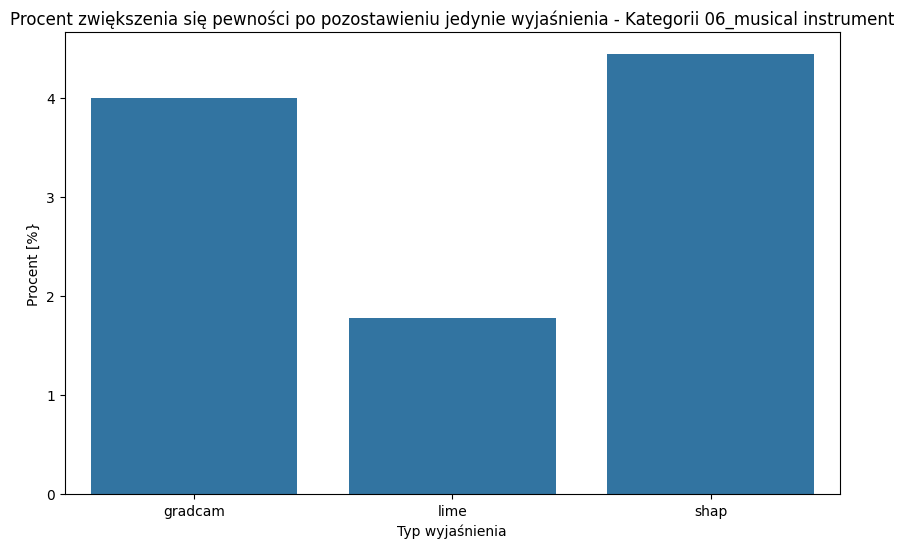
\includegraphics[width=.9\textwidth]{img/base_confidence_womask_percent_music}
		\caption{Procent zwiększenia się pewności po pozostawieniu jedynie wyjaśnienia - Kategoria Instrument}  \label{rys:base_confidence_womask_percent_music}
	\end{minipage}
	\begin{minipage}[b]{0.3\textwidth}
		\centering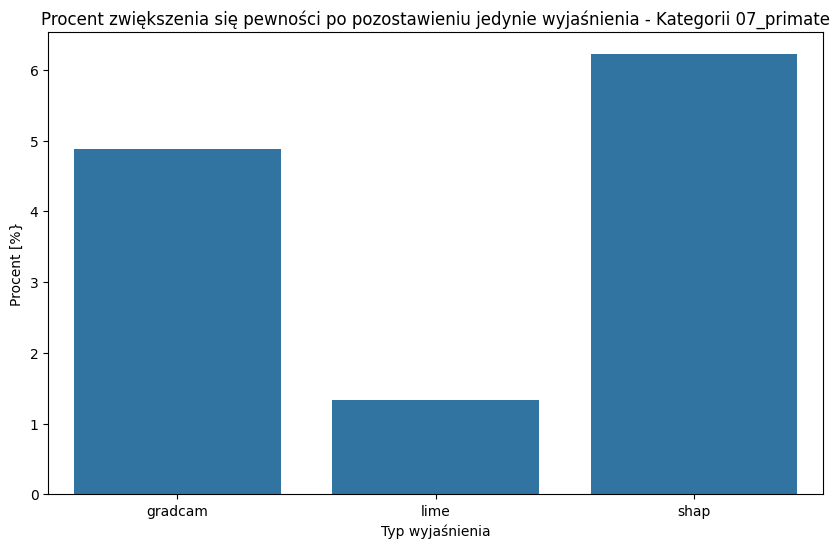
\includegraphics[width=.9\textwidth]{img/base_confidence_womask_percent_primate}
		\caption{Procent zwiększenia się pewności po pozostawieniu jedynie wyjaśnienia - Kategoria Primate}  \label{rys:base_confidence_womask_percent_primate}
	\end{minipage}
	\begin{minipage}[b]{0.3\textwidth}
		\centering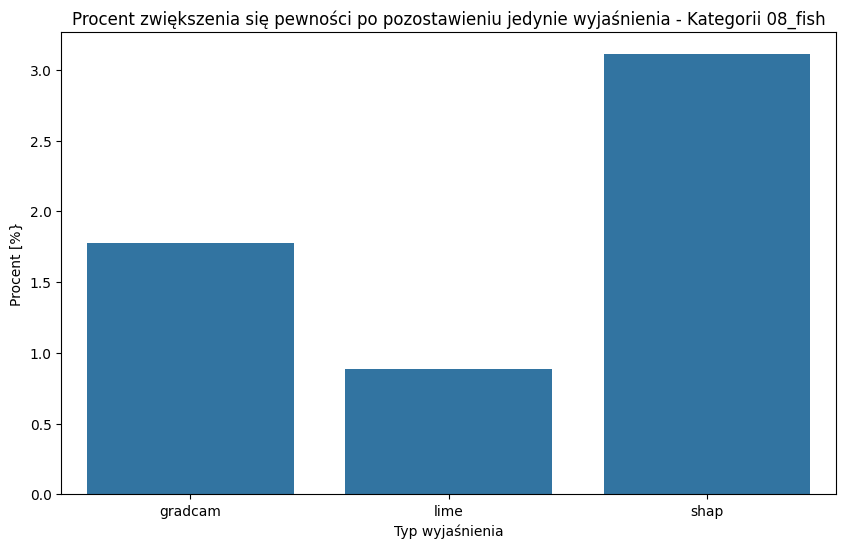
\includegraphics[width=.9\textwidth]{img/base_confidence_womask_percent_fish}
		\caption{Procent zwiększenia się pewności po pozostawieniu jedynie wyjaśnienia - Kategoria Fish}  \label{rys:base_confidence_womask_percent_fish}
	\end{minipage}
\end{figure}

We prawie wszystkich kategoriach po pozostawieniu jedynie obszaru wyjaśnienia LIME posiada najniższy procent zwiększenia się pewności.
Jedynym wyjątkiem jest kategoria Insect(\ref{rys:base_confidence_womask_percent_insect}) gdzie LIME posiada największy procent.
W kategoriach Carnivore, Fish, Dog, Reptile, Instrument, Vehicle, Prmiate, LIME jest znacząco mniejszy od pozostałych metod GradCAM oraz SHAP.

\subsection*{Wielkość obiektu}

\textbf{Analiza w zależności od wielkości obiektu}.
Przeanalizujemy teraz, jak metody XAI radzą sobie w identyfikacji istotnych cech obrazów w zależności od wielkości obiektów.
Porównamy wyniki IoU oraz zmiany pewności modelu dla małych, średnich oraz dużych obiektów.
Celem jest zrozumienie, jak wielkość obiektu wpływa na skuteczność wyjaśnień generowanych przez różne metody.
małe obiekty definiujemy jako obiekty zajmujące mniej niż 25\% obrazu, średnie mniej niż 50\%, natomiast duże to ponad 50\%.

\textbf{IoU}
\begin{figure}
	\centering
	\begin{minipage}[b]{0.3\textwidth}
		\centering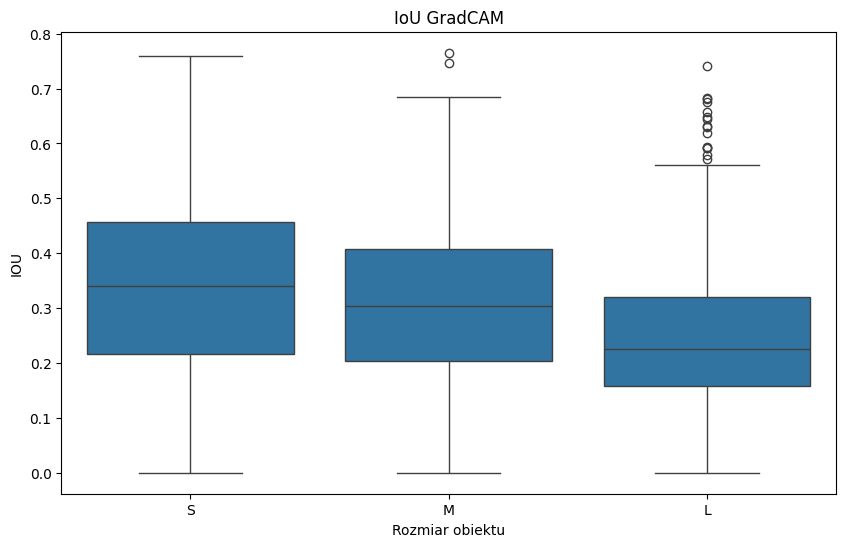
\includegraphics[width=.9\textwidth]{img/size_iou_gradcam}
		\caption{Wartość IoU wyjaśnień dla GradCAM}  \label{rys:size_iou_gradcam}
	\end{minipage}
	\begin{minipage}[b]{0.3\textwidth}
		\centering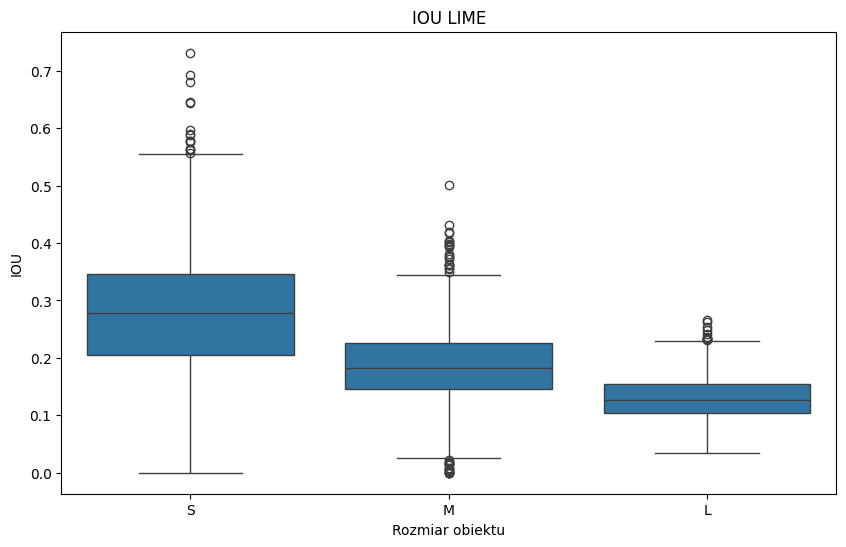
\includegraphics[width=.9\textwidth]{img/size_iou_lime}
		\caption{Wartość IoU wyjaśnień dla LIME}  \label{rys:size_iou_lime}
	\end{minipage}
	\begin{minipage}[b]{0.3\textwidth}
		\centering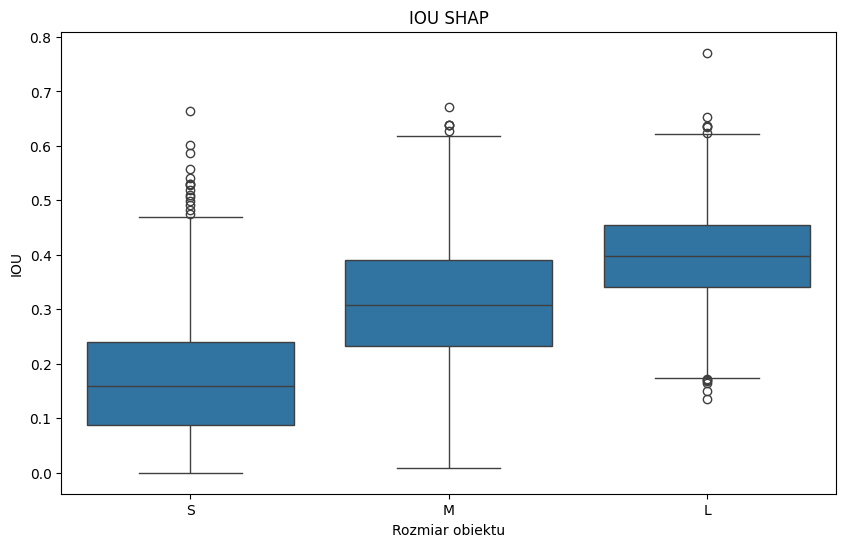
\includegraphics[width=.9\textwidth]{img/size_iou_shap}
		\caption{Wartość IoU wyjaśnień dla SHAP}  \label{rys:size_iou_shap}
	\end{minipage}
\end{figure}

\textbf{Zmaina pewności przy usunięciu obszarów wyjaśnienia}
\begin{figure}
	\centering
	\begin{minipage}[b]{0.3\textwidth}
		\centering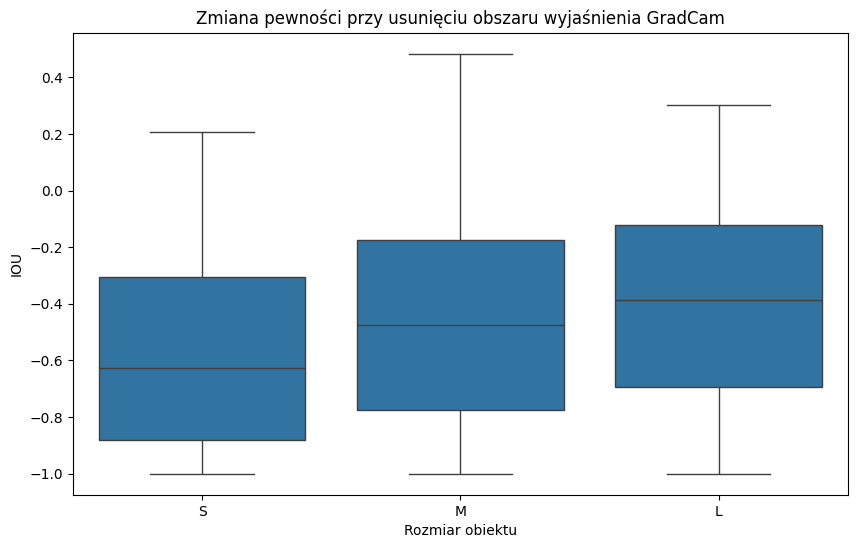
\includegraphics[width=.9\textwidth]{img/size_confidence_mask_gradcam}
		\caption{Zmiana pewności przy usunięciu obszarów wyjaśnienia dla GradCAM}  \label{rys:size_confidence_mask_gradcam}
	\end{minipage}
	\begin{minipage}[b]{0.3\textwidth}
		\centering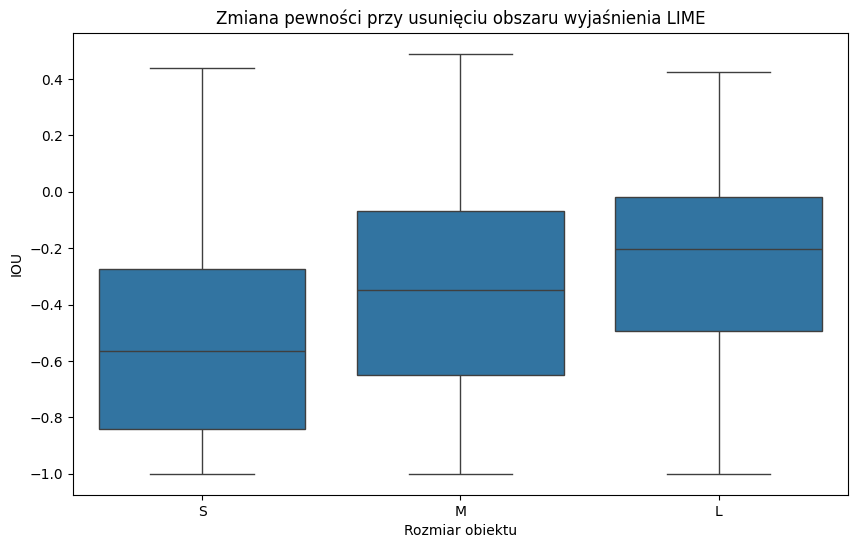
\includegraphics[width=.9\textwidth]{img/size_confidence_mask_lime}
		\caption{Zmiana pewności przy usunięciu obszarów wyjaśnienia dla LIME}  \label{rys:size_confidence_mask_lime}
	\end{minipage}
	\begin{minipage}[b]{0.3\textwidth}
		\centering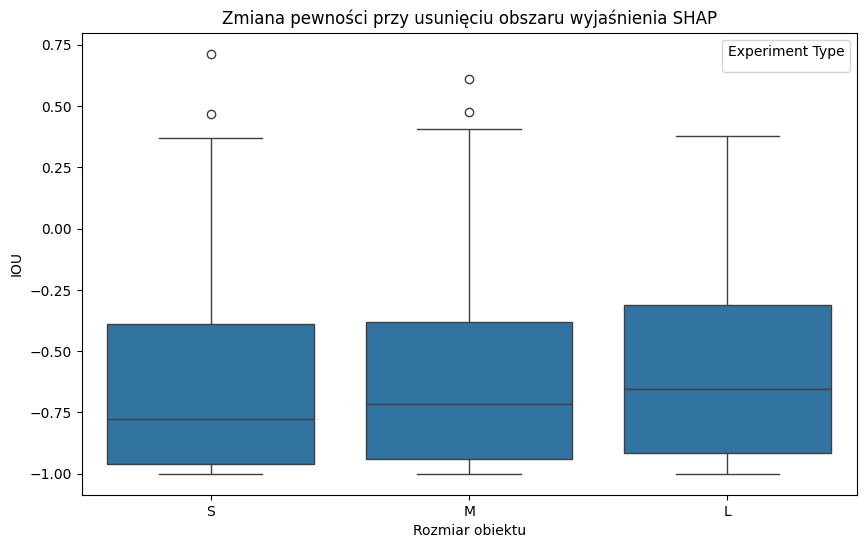
\includegraphics[width=.9\textwidth]{img/size_confidence_mask_shap}
		\caption{Zmiana pewności przy usunięciu obszarów wyjaśnienia dla SHAP}  \label{rys:size_confidence_mask_shap}
	\end{minipage}
\end{figure}

\textbf{Procent zwiększenia się pewności po pozostawienu jedynie wyjaśnienia}
\begin{figure}
	\centering
	\begin{minipage}[b]{0.3\textwidth}
		\centering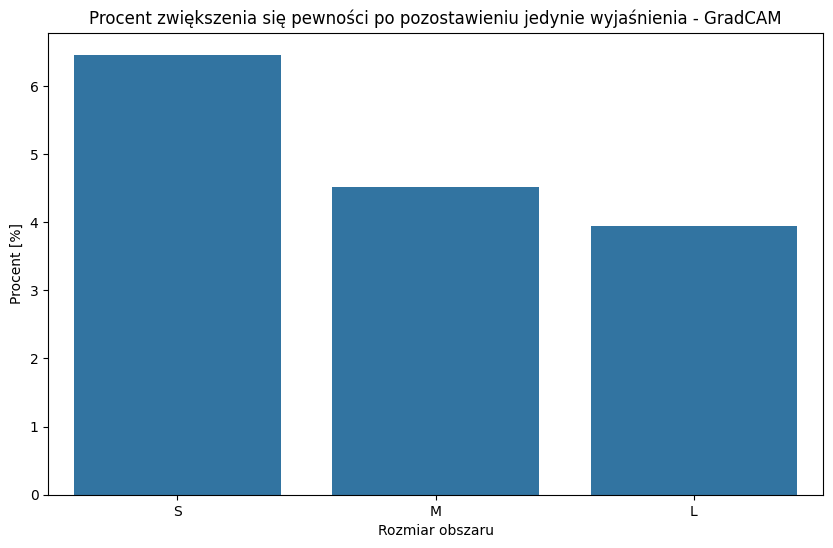
\includegraphics[width=.9\textwidth]{img/size_confidence_womask_percent_gradcam}
		\caption{Procent zwiększenia się pewności po pozostawieniu jedynie wyjaśnienia dla GradCAM}  \label{rys:size_confidence_womask_percent_gradcam}
	\end{minipage}
	\begin{minipage}[b]{0.3\textwidth}
		\centering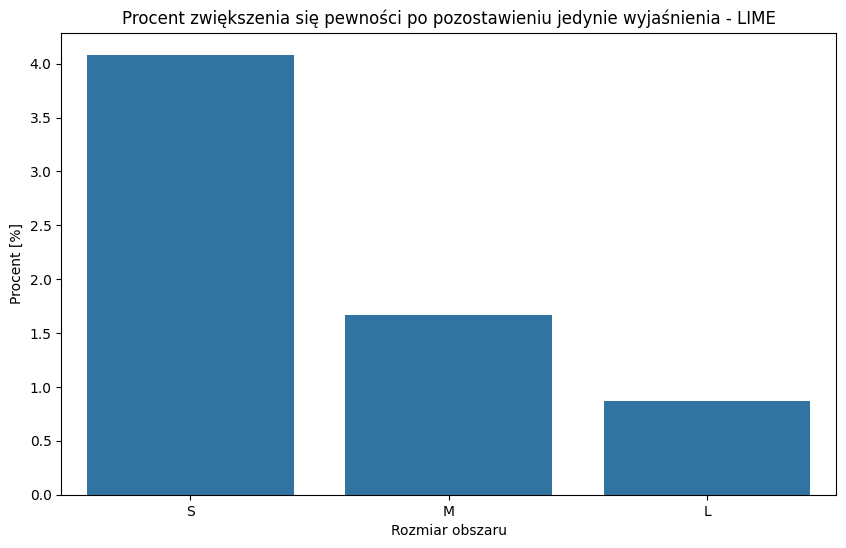
\includegraphics[width=.9\textwidth]{img/size_confidence_womask_percent_lime}
		\caption{Procent zwiększenia się pewności po pozostawieniu jedynie wyjaśnienia dla LIME}  \label{rys:size_confidence_womask_percent_lime}
	\end{minipage}
	\begin{minipage}[b]{0.3\textwidth}
		\centering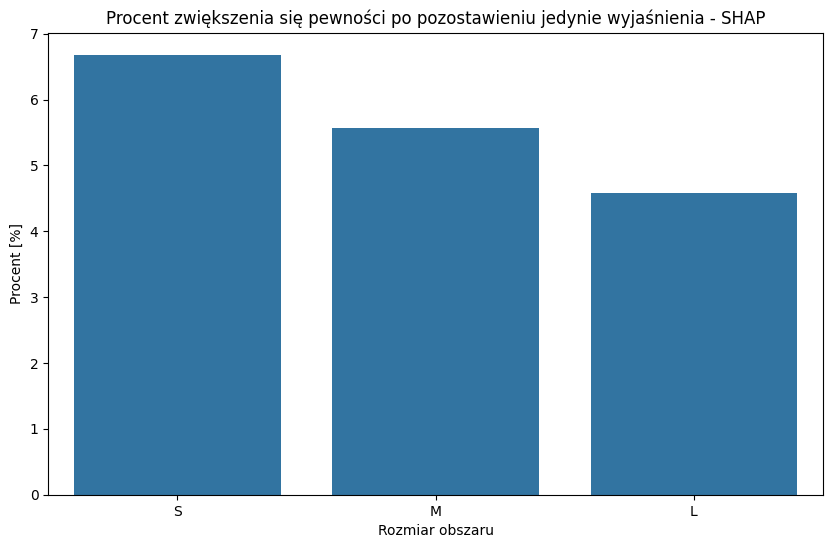
\includegraphics[width=.9\textwidth]{img/size_confidence_womask_percent_shap}
		\caption{Procent zwiększenia się pewności po pozostawieniu jedynie wyjaśnienia dla SHAP}  \label{rys:size_confidence_womask_percent_shap}
	\end{minipage}
\end{figure}

Jak widać ...

\textbf{Wnioski}
